\documentclass[10pt,twoside,a4paper]{article}
\usepackage{pslatex,palatino,avant,graphicx}
\usepackage[usenames,dvipsnames]{color}
\usepackage[margin=2cm]{geometry}
\usepackage{url}
\usepackage[square,sort]{natbib}

\usepackage{listings}
\lstset{ %
  backgroundcolor=\color{white},   % choose the background color; you must add \usepackage{color} or \usepackage{xcolor}
  basicstyle=\footnotesize,        % the size of the fonts that are used for the code
  breakatwhitespace=false,         % sets if automatic breaks should only happen at whitespace
  breaklines=true,                 % sets automatic line breaking
  captionpos=b,                    % sets the caption-position to bottom
  commentstyle=\color{LimeGreen},  % comment style
  % deletekeywords={...},            % if you want to delete keywords from the given language
  escapeinside={\%*}{*)},          % if you want to add LaTeX within your code
  extendedchars=true,              % lets you use non-ASCII characters; for 8-bits encodings only, does not work with UTF-8
  frame=single,                    % adds a frame around the code
  keepspaces=true,                 % keeps spaces in text, useful for keeping indentation of code (possibly needs columns=flexible)
  keywordstyle=\color{BlueGreen},  % keyword style
  % language=Java,                   % the language of the code
  % numbers=left,                    % where to put the line-numbers; possible values are (none, left, right)
  % numbersep=5pt,                   % how far the line-numbers are from the code
  % numberstyle=\tiny\color{Gray},   % the style that is used for the line-numbers
  rulecolor=\color{black},         % if not set, the frame-color may be changed on line-breaks within not-black text (e.g. comments (green here))
  showspaces=false,                % show spaces everywhere adding particular underscores; it overrides 'showstringspaces'
  showstringspaces=false,          % underline spaces within strings only
  showtabs=false,                  % show tabs within strings adding particular underscores
  stepnumber=2,                    % the step between two line-numbers. If it's 1, each line will be numbered
  stringstyle=\color{RubineRed},   % string literal style
  tabsize=2,                       % sets default tabsize to 2 spaces
  title=\lstname,                  % show the filename of files included with \lstinputlisting; also try caption instead of title
  aboveskip=1em,
  belowcaptionskip=0em,
  belowskip=0em
}

\usepackage{hyperref}
\hypersetup{
    colorlinks,
    citecolor=Violet,
    filecolor=black,
    linkcolor=MidnightBlue,
    urlcolor=MidnightBlue
}

% Definition of \maketitle
\makeatletter
\def\@maketitle{
\begin{center}

\includegraphics[width = 30mm]{images/logo.png}\\[2ex]
{\Huge \bfseries \sffamily \@title }\\[2ex]
{\Large  \@author}\\[4ex]
\@date\\%[8ex]
%
\includegraphics[width = 40mm]{images/logo.png}
\end{center}}
\makeatother

\begin{document}
\providecommand{\versionnumber}{0.1.10}
\title{ModelTest Manual v\versionnumber}
\author{Diego Darriba, David Posada, Alexandros Stamatakis, Tomas Flouris}
\date{\today}
\maketitle

\newcommand{\modeltest}{\emph{ModelTest-NG} }
\newcommand{\modeltestbin}{\emph{modeltest-cmd} }
\newcommand{\modeltestguibin}{\emph{modeltest-gui} }

\setcounter{tocdepth}{2}
\tableofcontents

\clearpage

\section{Overview}

{\modeltest} is a tool to carry out statistical selection of best-fit models of nucleotide substitution or amino acid replacement.
It implements five different model selection strategies: hierarchical and dynamical likelihood ratio tests (hLRT and dLRT), Akaike and Bayesian information criteria (AIC and BIC), and a decision theory method (DT).
It also provides estimates of model selection uncertainty, parameter importances and model-averaged parameter estimates, including model-averaged tree topologies.
{\modeltest} gathers features of {\em jModelTest 2} \citep{Darriba2013} and {\em ProtTest 3} \citep{Darriba2011}.

\subsection{Download}

The main project webpage is located at GitHub: \url{https://github.com/ddarriba/modeltest}.

New distributions of ModelTest-Light will be hosted in GitHub releases.
\begin{itemize}
  \item \url{https://github.com/ddarriba/modeltest/releases}
\end{itemize}

Please use the jModelTest discussion group for any question:
\begin{itemize}
  \item \url{http://groups.google.com/group/jmodeltest}.
\end{itemize}

%\subsection{Citation}

%When using {\modeltest} you should cite all these:

%\begin{itemize}
%\item xxx
%\end{itemize}

\subsection{Disclaimer}

{\footnotesize
This program is free software; you can redistribute it and/or modify it under the terms of the GNU General Public License as published by the Free Software Foundation;
either version 3 of the License, or (at your option) any later version. This program is distributed in the hope that it will be useful, but WITHOUT ANY WARRANTY;
without even the implied warranty of MERCHANTABILITY or FITNESS FOR A PARTICULAR PURPOSE. See the GNU General Public License for more details.
You should have received a copy of the GNU General Public License along with this program; if not, write to the Free Software Foundation, Inc., 59 Temple Place - Suite 330, Boston, MA 02111-1307, USA.
}

%%%%%%%%%%%%%%%%%%%%%%%%%%%%%%%%%%%%%%

{\footnotesize
\subsection{Last Updates}

\begin{itemize}

  \item 3 Mar 2016 Version 2.1.10 Revision 20160303
  \begin{itemize}
    \item xxx
  \end{itemize}

\end{itemize}


}

%%%%%%%%%%%%%%%%%%%%%%%%%%%%%%%%%%%%%%

\section{Getting Started}

\modeltest provides graphical and a command console interfaces.

\subsection{Compilation}

Sources can be compiled for every major Operating System, including Linux, Windows, and Mac OS X. For convenience, with each release you will find binaries for each of these systems.
Nonetheless, it might happen that for certain distributions only some of theme are available, for example if the realease fixes a bug affecting one single OS.

This tool is distributed under GPL v3 license. 
The source code is freely available at github repository: \url{https://github.com/ddarriba/modeltest}.

If you clone the repository, make sure to clone also libpll and pll-modules submodules with `--recursive` flag, or call `git submodule init --recursive` afterwards.

For most users, download the latest release and call the build script, {\em build.sh}. 
It should work correctly and (by default) compile all dependencies and place the final binaries under `build` directory.

\begin{itemize}
\item Run {\em build.sh} with no arguments for compiling all dependencies and modeltest in 3 flavors: {\em modeltest-ng} (command console execution), {\em modeltest-mpi} (MPI version), and {\em modeltest-gui} (graphical user interface). Note that you need QT 4 or 5 for compiling the GUI version.
\item Run {\em build.sh clean} for removing all object and output files.
\item Run {\em build.sh dist} for building a distribution package.
\end{itemize}

You can change the behaviour and the target directories in the static configuration section, at the beggining of the build script.

\begin{lstlisting}
# Static configuration                                                          
build_pll=yes            # build PLL                                            
build_modules=yes        # build PLL modules library                            
build_gui=yes            # build modeltest-gui                                  
dir_base=${PWD}          # base directory                                       
prefix=${dir_base}/build # output directory for modeltest                       
qmake_bin=qmake          # qmake binary (for GUI)
\end{lstlisting}

\begin{tabular}{lll}
  {\bf property} & {\bf default} & {\bf description} \\
  \hline
  build\_pll & yes & Build the pll dependency \\
  build\_modules & yes & Build the pll modules dependency \\
  build\_gui & yes & Build the graphical user interface \\
  dir\_base & current directory & Base directory \\
  prefix & {\em dir\_base}/build & Target directory \\
  qmake\_bin & qmake & qmake binary \\
\end{tabular}
\vspace{1em}

Note: QT utility, {\em qmake} can be also an absolute/relative path, e.g., {\em qmake\_bin=/usr/local/bin/qmake}.
For example, I used a custom distribution for OSX and the configuration line looks like this:

\begin{lstlisting}
qmake_bin=/usr/local/Cellar/qt/5.9.1/bin/qmake
\end{lstlisting}

\subsection{Example run}

\begin{enumerate}
\item Execute the following command line:

\begin{lstlisting}
$ ./modeltest-ng -i example-data/dna/tiny.fas -h uigf -f ef
\end{lstlisting}

This will test all 88 models (gamma models with 4 rate categories), and then perform the model selection using Akaike (AIC) and Bayesian (BIC) criteria.

See Section~\ref{sec:arguments} for information about supported arguments.

\item This will generate the following output:

\begin{enumerate}

\item Header:

\begin{lstlisting}
                             _      _ _            _      _   _  _____ 
                            | |    | | |          | |    | \ | |/ ____|
         _ __ ___   ___   __| | ___| | |_ ___  ___| |_   |  \| | |  __ 
        | '_ ` _ \ / _ \ / _` |/ _ \ | __/ _ \/ __| __|  | . ` | | |_ |
        | | | | | | (_) | (_| |  __/ | ||  __/\__ \ |_   | |\  | |__| |
        |_| |_| |_|\___/ \__,_|\___|_|\__\___||___/\__|  |_| \_|\_____|
--------------------------------------------------------------------------------

modeltest 0.1.0
Copyright (C) 2017 Diego Darriba, David Posada, Alexandros Stamatakis
License GPLv3+: GNU GPL version 3 or later <http://gnu.org/licenses/gpl.html>.
This is free software: you are free to change and redistribute it.
There is NO WARRANTY, to the extent permitted by law.

Written by Diego Darriba.
--------------------------------------------------------------------------------
\end{lstlisting}

\item System and configuration details:

\begin{lstlisting}
Physical cores: 2
Logical cores:  4
Memory:         3.57GB
Extensions:     AVX

\end{lstlisting}

\item Execution options:

\begin{lstlisting}
--------------------------------------------------------------------------------
Input data:
  MSA:        example-data/dna/aP6.fas
  Tree:       Maximum parsimony
    file:     -
  #taxa:      6
  #sites:     631
  #patterns:  28

Output:
  Log:           test.log
  Starting tree: test.tree
  Results:       test.out

Selection options:
  # dna schemes:      11
  # dna models:       88
  include model parameters:
    Uniform:         true
    p-inv (+I):      true
    gamma (+G):      true
    both (+I+G):     true
    fixed freqs:     true
    estimated freqs: true
    #categories:     4
  asc bias:           none
  epsilon (opt):      0.01
  epsilon (par):      0.01

Additional options:
  verbosity:        very low
  threads:          1/2
  RNG seed:         12345
  subtree repeats:  enabled
--------------------------------------------------------------------------------
modeltest-ng was called as follows:
>> src/modeltest-ng -i example-data/dna/aP6.fas -h uifg -f fe -o test
\end{lstlisting}

\item Real time optimization results (progress):

\begin{lstlisting}
Partition 1/1

 ----ID---  ----MODEL---- ---Time--- -Elapsed--- -------LnL------- -Alpha- -P-inv-
    1/88   JC             0h:00:00   0h:00:00           -1115.1193       -       -
    2/88   JC+I           0h:00:00   0h:00:00           -1103.3444       -  0.9082
    3/88   JC+G           0h:00:00   0h:00:00           -1106.6136  0.0200       -
    4/88   JC+I+G         0h:00:00   0h:00:00           -1103.6235  1.1674  0.8542
    5/88   F81            0h:00:00   0h:00:00           -1065.0339       -       -
    6/88   F81+I          0h:00:00   0h:00:00           -1053.6319       -  0.9032
    7/88   F81+G          0h:00:00   0h:00:00           -1056.6126  0.0200       -
    8/88   F81+I+G        0h:00:00   0h:00:00           -1053.8953  1.1494  0.8460

...

   85/88   GTR            0h:00:00   0h:00:01           -1063.2358       -       -
   86/88   GTR+I          0h:00:00   0h:00:01           -1051.9056       -  0.9001
   87/88   GTR+G          0h:00:00   0h:00:01           -1054.7872  0.0200       -
   88/88   GTR+I+G        0h:00:00   0h:00:01           -1052.1689  1.1396  0.8417
 ----ID---  ----MODEL---- ---Time--- -Elapsed--- -------LnL------- -Alpha- -P-inv-

Computation of likelihood scores completed. It took 0h:00:01
\end{lstlisting}

\item Selected Information Criteria (best model and all models sorted according to each criterion):

\begin{lstlisting}
BIC       model              K            lnL          score          delta    weight
--------------------------------------------------------------------------------
       1  F81+I              4     -1053.6319      2191.0788         0.0000    0.8565
       2  HKY+I              5     -1053.1557      2196.5737         5.4949    0.0549
       3  F81+G              4     -1056.6126      2197.0401         5.9613    0.0435
       4  F81+I+G            5     -1053.8953      2198.0529         6.9741    0.0262
       5  TrN+I              6     -1052.6019      2201.9134        10.8346    0.0038
       6  TPM2uf+I           6     -1052.6600      2202.0296        10.9507    0.0036
       7  HKY+G              5     -1056.0996      2202.4615        11.3827    0.0029
       8  TPM3uf+I           6     -1052.9534      2202.6164        11.5376    0.0027
       9  TPM1uf+I           6     -1053.0742      2202.8579        11.7791    0.0024
      10  HKY+I+G            6     -1053.4340      2203.5777        12.4988    0.0017
--------------------------------------------------------------------------------
Best model according to BIC
---------------------------
Model:              F81+I
lnL:                -1053.6319
Frequencies:        0.4253 0.1506 0.2010 0.2232
Subst. Rates:       1.0000 1.0000 1.0000 1.0000 1.0000 1.0000
Inv. sites prop:    0.9032
Gamma shape:        -
Score:              2191.0788
Weight:             0.8565
---------------------------
Parameter importances
---------------------------
P.Inv:              0.9244
Gamma:              0.0471
Gamma-Inv:          0.0282
Frequencies:        1.0000
---------------------------
Model averaged estimates
---------------------------
P.Inv:              0.9031
Alpha:              0.0200
Alpha-P.Inv:        1.1502
P.Inv-Alpha:        0.8459
Frequencies:        0.4253 0.1506 0.2010 0.2232

Commands:
  > phyml  -i example-data/dna/aP6.fas -m 000000 -f m -v e -a 0 -c 1 -o tlr
  > raxmlHPC-SSE3 -s example-data/dna/aP6.fas -c 1 -m GTRCATIX --JC69 -n EXEC_NAME -p PARSIMONY_SEED
  > paup -s example-data/dna/aP6.fas
  > iqtree -s example-data/dna/aP6.fas -m F81+I
\end{lstlisting}

\item Consensus tree of the optimized phylogenies using the criterion weights (only for {\bf ML topologies}):

\begin{lstlisting}
  There are 2 different topologies
  Topologies written to output.topos

  topo_id   models_count   bic_support   aic_support   aicc_support
  -----------------------------------------------------------------
        1             37       0.95897       0.66064       0.66964
        2             51       0.04103       0.33936       0.33036

  extended majority-rule consensus: ((P4,(P6,P1)[1.00000])[0.95897],P5,(P2,P3)[1.00000]);
  strict consensus: ((P6,P1)[1.00000],P4,P5,(P2,P3)[1.00000]);
\end{lstlisting}

\end{enumerate}
\end{enumerate}


%%%%%%%%%%%%%%%%%%%%%%%%%%%%%%%%%%%%%%%%%%%%%%%%%%%%%%%%%%%

\section{Graphical User Interface}
\label{sec:gui}

\subsection{Launching the Graphical User Interface}

Running {\modeltestguibin} with no arguments launches the graphical interface.
The following window will show on the screen:

\begin{center}
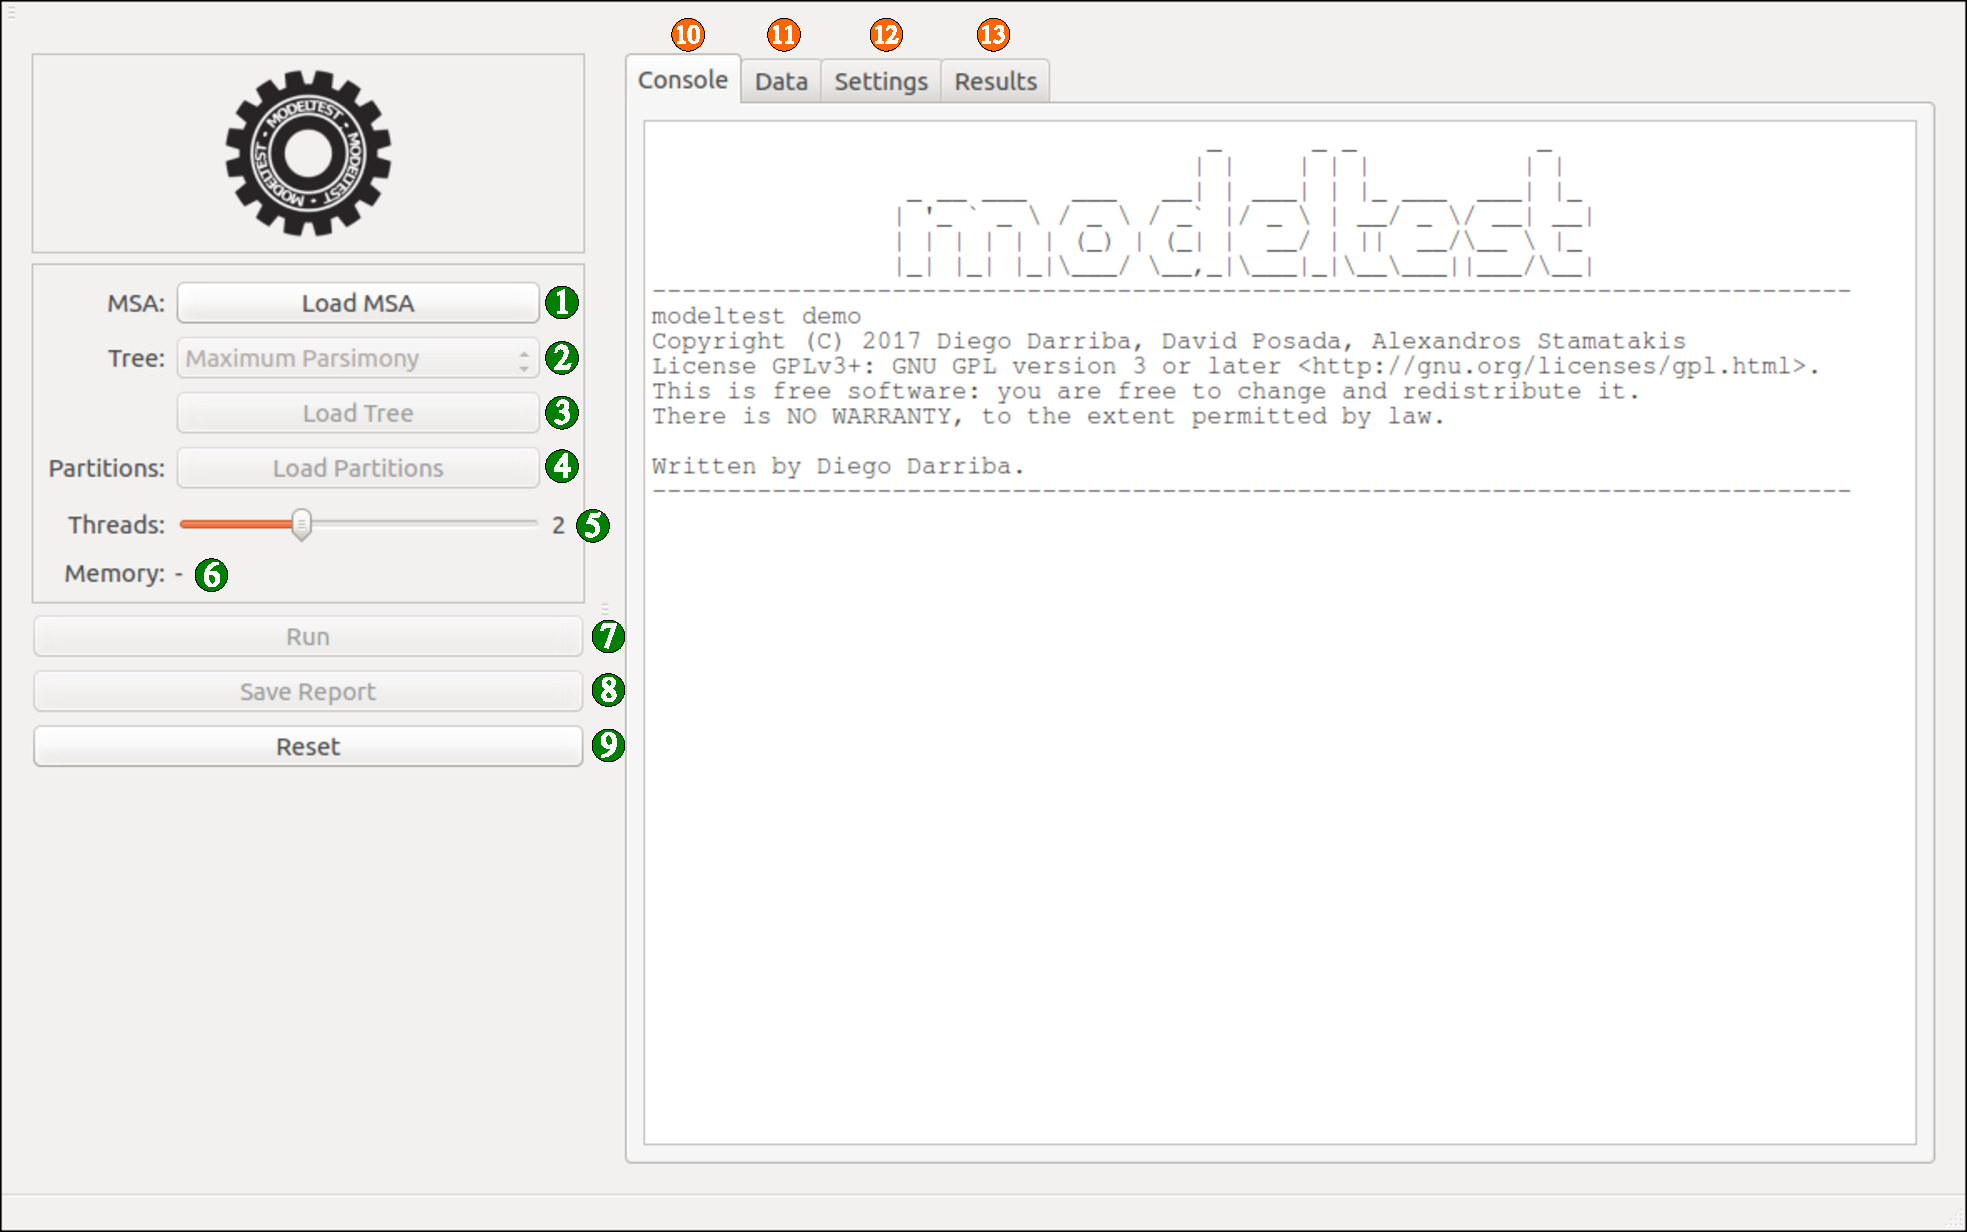
\includegraphics[width=.9\textwidth]{images/main-window}
\end{center}

\begin{tabular}{l p{.7\textwidth}}
  \color{ForestGreen}1 & Load an MSA file in PHYLIP or FASTA format \\
  \color{ForestGreen}2 & Select the phylogenetic tree for each model \\
  \color{ForestGreen}3 & Load a fixed or starting tree in NEWICK format (optional) \\
  \color{ForestGreen}4 & Load a partitioning scheme file in RAxML format (optional) \\
  \color{ForestGreen}5 & Select the number of concurrent threads to use \\
  \color{ForestGreen}6 & Displays the estimated amount of memory needed as a function of the MSA size and the number of threads \\
  \hline
  \color{ForestGreen}7 & Start model selection process \\
  \color{ForestGreen}8 & Save the results report in a file \\
  \color{ForestGreen}9 & Reset the interface \\
  \hline
  \color{RedOrange}10 & Pane containing the main output console \\
  \color{RedOrange}11 & Pane containing data description \\
  \color{RedOrange}12 & Pane containing the model selection configuration \\
  \color{RedOrange}13 & Pane containing the model selection results \\
\end{tabular}

\subsection{Custom settings}

The settings tab ({\color{RedOrange}12}) allows to change the model optimization settings.
Although the default settings are the most commonly used, you might want to use different ones for your own purposes.

\begin{center}
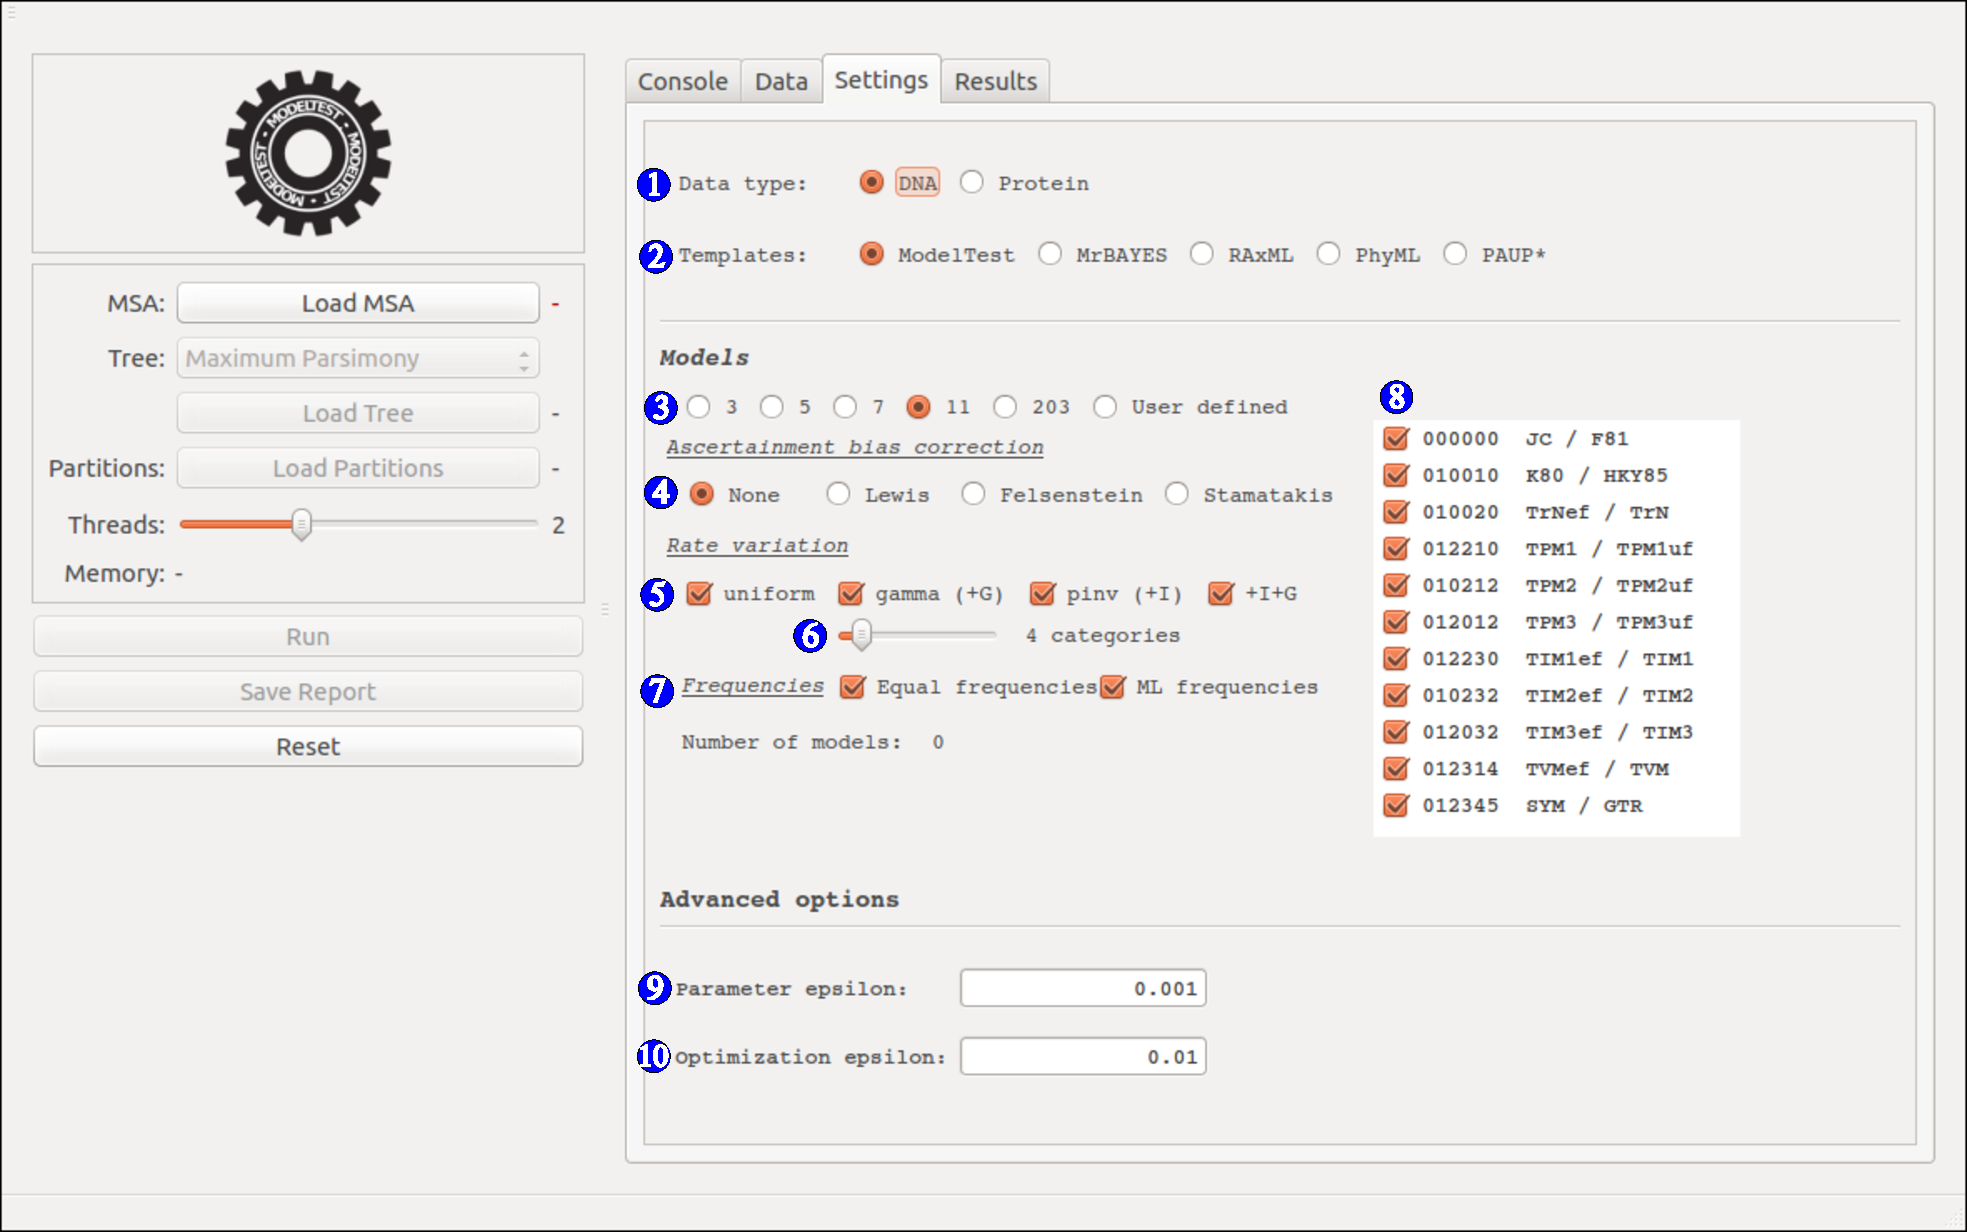
\includegraphics[width=.9\textwidth]{images/lkl-settings}
\end{center}

\begin{tabular}{l p{.7\textwidth}}
  \color{Blue}1  & Data type (DNA or amino acids) \\
  \color{Blue}2  & Use only models available in a particular phylogenetic inference tool \\
  \color{Blue}3  & Use \emph{a priori} defined subset of substitution schemes \\
  \color{Blue}4  & Correct models for ascertainment bias \\
  \color{Blue}5  & Include models of rate variation among sites \\
  \color{Blue}6  & Select the number of discrete rate categories for Gamma model of rate variation \\
  \color{Blue}7  & Include equal/model-defined or ML/empirical frequencies \\
  \color{Blue}8  & Select individual candidate models \\
  \hline
  \color{Blue}9  & Tolerance for single parameter optimization \\
  \color{Blue}10 & Global tolerance for model optimization \\
\end{tabular}

\subsection{Example}

If you want to start running a small example, press {\emph Ctrl+O} in the main window.
Select a MSA file from `example-data/nucleic' or `example-data/proteic' in the dialog, either in FASTA or PHYLIP format.
Press {\emph Ctrl+T} and select the corresponding tree file in the dialog, in NEWICK format.
Press {\emph Ctrl+R} and enjoy the execution.

%%%%%%%%%%%%%%%%%%%%%%%%%%%%%%%%%%%%%%%%%%%%%%%%%%%%%%%%%%%

\section{Command Line Arguments}
\label{sec:arguments}

\subsection{Overview}

\subsubsection{Main Arguments}

\begin{tabular}{rllp{.6\textwidth}}
  \hline
  \texttt{-d} & \texttt{--datatype}   & \bf{nt},\bf{aa} & Data type is `nt' for nucleotide (default), `aa' for amino-acid sequences. \\
  \texttt{-i} & \texttt{--input}      & {\em filename} & Input MSA file in FASTA or sequential PHYLIP format. Check section~\ref{sec:arg:input} \\
  \texttt{-t} & \texttt{--topology}   & {\em topology\_type}. & Check section~\ref{sec:arg:topo} \\
               && \bf{ml}             & maximum likelihood \\
               && \bf{mp}             & maximum parsimony (default)\\
               && \bf{fixed-ml-jc}    & fixed maximum likelihood (JC) \\
               && \bf{fixed-ml-gtr}   & fixed maximum likelihood (GTR) \\
               && \bf{random}         & random generated tree \\
               && \bf{user}           & fixed user defined (requires -u argument) \\
  \texttt{-u} & \texttt{--utree}      & {\em filename} & User-defined tree in NEWICK format. Check section~\ref{sec:arg:topo}\\
  \texttt{-q} & \texttt{--partitions} & {\em filename} & Partitions filename in RAxML format. Check section~\ref{sec:arg:parts} \\
  \texttt{-o} & \texttt{--output}     & {\em filename} & Pipes the output into a file \\
  \texttt{-p} & \texttt{--processes}  & {\em number\_of\_threads} & Number of concurrent threads \\
  \texttt{-r} & \texttt{--rngseed}    & {\em seed} & Sets the seed for the random number generator \\
  \hline
\end{tabular}

\subsubsection{Candidate Models}

  \begin{tabular}{rllp{.6\textwidth}}
    \hline
    \texttt{-a} & \texttt{--asc-bias} & algorithm[:values] & Includes ascertainment bias correction. Check section~\ref{sec:ascbias} for more details \\
                                     &&&  {\bf lewis}: Lewis (2001) \\
                                     &&&  {\bf felsenstein}: Felsenstein (requires number of invariant sites) \\
                                     &&&  {\bf stamatakis}: Leaché et al. (2015) (requires invariant sites composition) \\
     \texttt{-f} & \texttt{--frequencies} & [ef]           & Sets the candidate models frequencies \\
                                     &&& {\bf e}: Estimated - maximum likelihood (DNA) / empirical (AA) \\
                                     &&& {\bf f}: Fixed - equal (DNA) / model defined (AA) \\
     \texttt{-h} & \texttt{--model-het} & [uigf] & Sets the candidate models rate heterogeneity \\
                                     &&& {\bf u}: Uniform \\
                                     &&& {\bf i}: Proportion of invariant sites (+I) \\
                                     &&& {\bf g}: Discrite Gamma rate categories (+G) \\
                                     &&& {\bf f}: Both +I and +G (+I+G) \\
     \texttt{-m} & \texttt{--models}  & {\em list} & Sets the candidate model matrices separated by commas \\
                                      && dna: & JC HKY TrN TPM1 TPM2 TPM3 TIM1 TIM2 TIM3 TVM GTR \\
                                      && protein: & DAYHOFF LG DCMUT JTT MTREV WAG RTREV CPREV VT BLOSUM62 MTMAM MTART MTZOA PMB HIVB HIVW JTTDCMUT FLU STMTREV \\
    \texttt{-s} & \texttt{--schemes}  & {\em number\_of\_schemes} & Number of DNA substitution schemes. \\
                                      &&& {\bf 3}: JC, HKY, GTR \\
                                      &&& {\bf 5}: JC, HKY, TrN, TPM1, GTR \\
                                      &&& {\bf 7}: JC, HKY, TrN, TPM1, TIM1, TVM, GTR \\
                                      &&& {\bf 11}: All models defined in Sec~\ref{subsec:models} \\
                                      &&& {\bf 203}: All possible GTR submatrices \\
    \texttt{-T} & \texttt{--template} & {\em tool} & Sets candidate models according to a specified tool \\
                  && {\bf raxml}      & RAxML (DNA 3 schemes / AA full search) \\
                  && {\bf phyml}      & PhyML (DNA full search / 14 AA matrices) \\
                  && {\bf mrbayes}    & MrBayes (DNA 3 schemes / 8 AA matrices) \\
                  && {\bf paup}       & PAUP* (DNA full search / AA full search) \\
    \hline
  \end{tabular}

\subsubsection{Other options}

  \begin{tabular}{rllp{.6\textwidth}}
    \hline
      & \texttt{--eps} & {\em epsilon\_value}    & Sets the model optimization epsilon \\
      & \texttt{--tol} & {\em tolerance\_value}  & Sets the parameter optimization tolerance \\
      & \texttt{--smooth-frequencies}   & & Forces frequencies smoothing \\
   \texttt{-H} & \texttt{--no-compress} & & Disables pattern compression. \modeltest ignores if there are missing states \\
   \texttt{-v} & \texttt{--verbose} & & Run in verbose mode \\
      & \texttt{--help}    & & Display this help message and exit \\
      & \texttt{--version} & & Output version information and exit \\
  \end{tabular}

\section{Model Optimization Settings}
\label{sec:optsettings}

\subsection{Input data}
\label{sec:arg:input}

The main and only required argument is the multiple sequence alignment file ($-i$ argument).
\modeltest supports PHYLIP and FASTA format.
All sequences must be alignned and have thus have the same sequence length.

PHYLIP format starts with a header line containing 2 integer values corresponding to the number of sequences and the sequence length.
The following lines are the individual taxa followed by the corresponding sequence.
Taxon names and sequences must \emph{not} contain whitespaces.
If that is the case in your alignment, please remove or replace every white space with any arbitrary character, such for example an underscore.

Please note that at this moment \modeltest does not support interleaved PHYLIP format.

{
\begin{verbatim}
TAXA_COUNT SEQ_LENGTH
TAXON_NAME_1 SEQUENCE_1
TAXON_NAME_2 SEQUENCE_2
TAXON_NAME_3 SEQUENCE_3
...
TAXON_NAME_N SEQUENCE_N
\end{verbatim}
}

Example:

{
\begin{verbatim}
5 20
taxon1 acgctatcgcgatcgatagc
taxon2 aaactagggcgatcgatagg
taxon3 acactatcg---tcgatagg
taxon4 acgctatcg---ccgatagg
taxon5 acgctaacgcgaacgttatc
\end{verbatim}
}

FASTA format does not contain any header, and it is formatted as a list of the sequences,
each of them covering 2 lines: the taxon name, and the sequence.

{
\begin{verbatim}
>TAXON_NAME_1
SEQUENCE_1
>TAXON_NAME_2
SEQUENCE_2
>TAXON_NAME_3
SEQUENCE_3
...
>TAXON_NAME_N
SEQUENCE_N
\end{verbatim}
}

The example below is analogous to the previous example in PHYLIP format:

{
\begin{verbatim}
>taxon1
acgctatcgcgatcgatagc
>taxon2
aaactagggcgatcgatagg
>taxon3
acactatcg---tcgatagg
>taxon4
acgctatcg---ccgatagg
>taxon5
acgctaacgcgaacgttatc
\end{verbatim}
}

\subsection{Models of evolution}
\label{subsec:models}

\modeltest implementes all 203 types of time-reversible substitution matrices,
with when combined with unequal/equal base frequencies,
gamma-distributed among-site rate variation and a proportion of invariable sites
makes a total of 1624 models.
Some of the models have received names:

\vspace{1em}
\begin{tabular}{l l l l l l}
\hline
{\bf Model} & {\bf Reference} & {\bf Free}   & {\bf Base}  & {\bf Substitution rates} & {\bf Substitution} \\
            &                 & {\bf param.} & {\bf freq.} &                          & {\bf code} \\
\hline
JC & \citep{Jukes-1969} & 0 & equal & AC=AG=AT=CG=CT=GT & 000000 \\
\hline
F81 & \citep{Felsenstein-1981} & 3 & unequal & AC=AG=AT=CG=CT=GT & 000000 \\
\hline
K80 & \citep{Kimura-1980} & 1 & equal & AC=AT=CG=GT;AG=GT & 010010 \\
\hline
HKY & \citep{Hasegawa-1985} & 4 & unequal & AC=AT=CG=GT;AG=GT & 010010 \\
\hline
TrNef & \citep{Tamura-1993} & 2 & equal & AC=AT=CG=GT;AG;GT & 010020 \\
\hline
TrN & \citep{Tamura-1993} & 5 & unequal & AC=AT=CG=GT;AG;GT & 010020 \\
\hline
TPM1 & =K81 \citep{Kimura-1981} & 2 & equal & AC=GT;AG=CT;AT=CG & 012210 \\
\hline
TPM1uf & \citep{Kimura-1981} & 5 & unequal & AC=GT;AG=CT;AT=CG & 012210 \\
\hline
TPM2 & & 2 & equal & AC=AT;CG=GT;AG=CT & 010212 \\
\hline
TPM2uf & & 5 & unequal & AC=AT;CG=GT;AG=CT & 010212 \\
\hline
TPM3 & & 2 & equal & AC=AT;AG=GT;AG=CT & 012012 \\
\hline
TPM3uf & & 5 & unequal & AC=CG;AT=GT;AG=CT & 012012 \\
\hline
TIM1 & \citep{Posada-2003} & 3 & equal & AC=GT;AT=CG;AG;CT & 012230 \\
\hline
TIM1uf & \citep{Posada-2003} & 6 & unequal & AC=GT;AT=CG;AG;CT & 012230 \\
\hline
TIM2 & & 3 & equal & AC=AT;CG=GT;AG;CT & 010232 \\
\hline
TIM2uf & & 6 & unequal & AC=AT;CG=GT;AG;CT & 010232 \\
\hline
TIM3 & & 3 & equal & AC=CG;AT=GT;AG;CT & 012032 \\
\hline
TIM3uf & & 6 & unequal & AC=CG;AT=GT;AG;CT & 012032 \\
\hline
TVMef & \citep{Posada-2003} & 4 & equal & AC;CG;AT;GT;AG=CT & 012314 \\
\hline
TVM & \citep{Posada-2003} & 7 & unequal & AC;CG;AT;GT;AG=CT & 012314 \\
\hline
SYM & \citep{Zharkikh-1994} & 5 & equal & AC;CG;AT;GT;AG;CT & 012345 \\
\hline
GTR & =REV \citep{Tavare-1986} & 8 & unequal & AC;CG;AT;GT;AG;CT & 012345 \\
\hline
\end{tabular}
\vspace{1em}

\modeltest includes the empirical amino acid matrices described in the table below.
If you expect a very long runtime according to the size of your data,
it is recommended to select {\em a priori} a sensible set of candidate matrices instead of evaluating all the available ones
(e.g., discarding those matrices estimated from different data).

\vspace{1em}
\begin{tabular}{ll}
  \hline
  {\bf Model} & {\bf Description} \\
  \hline
  Dayhoff &	General matrix~\citep{dayhoff1978} \\
  \hline
  JTT &	General matrix~\citep{jones1992} \\
  \hline
  DCMut/JTT-DCMut & Revised Dayhoff and JTT matrices~\citep{kosiol2005} \\
  \hline
  WAG & General matrix~\citep{whelan2001} \\
  \hline
  VT & General matrix~\citep{muller2000}  \\
  \hline
  cpREV & Chloroplast matrix~\citep{adachi2000} \\
  \hline
  rtREV & Retrovirus~\citep{dimmic2002} \\
  \hline
  stmtREV & Streptophyte mitochondrial land plants~\citep{liu2014} \\
  \hline
  mtArt & Mitochondrial Arthropoda~\citep{abascal2007} \\
  \hline
  mtMam & Mitochondrial Mammals~\citep{yang1998} \\
  \hline
  mtREV & Mitochondrial Verterbrate~\citep{adachi1996} \\
  \hline
  mtZoa & Mitochondrial Metazoa (Animals)~\citep{rota2009} \\
  \hline
  HIVb/HIVw & HIV matrices ~\citep{nickle2007} \\
  \hline
  LG & General matrix~\citep{le2008} \\
  \hline
  Blosum62 & BLOcks SUbstitution Matrix~\citep{henikoff1992} \\
  \hline
  PMB & Revised Blosum matrix~\citep{veerassamy2003} \\
  \hline
  FLU & Influenza virus~\citep{dang2010} \\
  \hline
  LG4M & 4-matrix mixture model with discrete $\Gamma$ rates ~\citep{le2012} \\
  \hline
  LG4X & 4-matrix mixture model with free rates~\citep{le2012} \\
  \hline
\end{tabular}

\subsection{Topology type}
\label{sec:arg:topo}

By default, \modeltest optimizes each single model using a fixed Maximum-Parsimony topology
with Maximum-Likelihood optimized branch lengths.
However, it allows other tree optimization techniques.
The topology type can be selected with $-t$ argument and it accepts the following values:

\begin{itemize}
  \item {\bf ml:} Optimize topology and branch lengths for each model
  \item {\bf fixed-ml-jc:} Build a ML topology with Jukes-Cantor model and fixes it for every other.
  \item {\bf fixed-ml-gtr:} Build a ML topology with GTR model and fixes it for every other.
  \item {\bf random:} Use a fixed randomly generated tree.
  \item {\bf user:} Use fixed user-defined topology
\end{itemize}

In addition to that, you can set a custom tree topology using $-u$ argument, followed by a file containing the tree in NEWICK format.
\modeltest works only with unrooted topologies, so if the user-defined tree is rooted, it will be automatically unrooted.
This argument is mandatory if the tree type was set to {\emph user}, and optional for ML trees.
In the latter case, the custom-defined tree is used as starting point for the ML optimization, while otherwise \modeltest uses a MP tree.

A {\emph random} tree topology can be interesting if one wants to measure how sensitive is the model selection process to the tree topology.
If you want to test several different random trees, do not forget to use different RNG seeds ($-r$ argument).


\subsection{Partitioning scheme}
\label{sec:arg:parts}

\modeltest is able to select individual models of evolution for each partition defined on the data set ($-q$ argument).
The partitioning scheme used may be defined in a file using RAxML-like format, where each partition is defined by one line in the file as follows:

{
\begin{verbatim}
DATA_TYPE, PARTITION_NAME = PARTITION_SITES
\end{verbatim}
}

Where:

\begin{itemize}
  \item {\bf DATA\_TYPE} can be {\emph DNA} or {\emph PROTEIN}
  \item {\bf PARTITION\_NAME} is an arbitrary name for each partition
  \item {\bf PARTITION\_SITES} is the subset of sites that belong to the partition.
        They can be contiguous (e.g.,1-1000), or defined in several sections (e.g., $1-1000,2500-3000$).
        Additionally, one can specify a stride.
        For example, a partition covering all first codon positions in the first 1,000 sites is defined as $1-1000 \backslash 3$,
        second codon position is $2-1000 \backslash 3$, and third $3-1000 \backslash 3$.
        Second and third codon positions together would be $2-1000 \backslash 3,3-1000 \backslash 3$.
\end{itemize}

For example:

{
\begin{verbatim}
  DNA, GENE1 = 1-800
  DNA, GENE2_1 = 1701-2400\3
  DNA, GENE2_2 = 1702-2400\3
  DNA, GENE2_3 = 1703-2400\3
  DNA, GENE3 = 801-1700,2401-2500
\end{verbatim}
}

Partitions do not need to cover all sites in the MSA.
Every site which does not belong to any partition is just ignored.
Also, there must not be overlapping partitions (i.e., it is not allowed a site to belong to more than one partition).

\subsection{Ascertainment Bias Correction}
\label{sec:ascbias}

{\modeltest} incorporates 3 algorithms for including ascertainment bias correction in the candidate models.

Let $c$ be the sum of likelihoods ({\bf not} log-likelihoods) of the {\emph `dummy'}, or virtual invariant sites containing each of the states (eq.~\ref{eq:sumdummy}):,
$n$ is the number of sites,
$s$ is the number of states,
$\omega$ is the number of invariant sites,
and $\omega_i$ is the number of invariant sites for state $i$.

\begin{equation}
  \label{eq:sumdummy}
  c = \sum\limits_{i}^{s}L(s)
\end{equation}

\begin{itemize}
  \item Lewis (Lewis, 2001)
    \begin{equation}
      ln(L) = \sum\limits_{i}^{n}ln(L_i) - n \cdot ln(1-c)
    \end{equation}
  \item Felsenstein (Felsenstein, xx)
    \begin{equation}
      ln(L) = \sum\limits_{i}^{n}ln(L_i) + \omega \cdot ln(c)
    \end{equation}
  \item Stamatakis (Leach\'e et al. 2015)
    \begin{equation}
      ln(L) = \sum\limits_{i}^{n}ln(L_i) + \sum\limits_{j}^{s} \omega_j \cdot ln(L(j))
    \end{equation}
\end{itemize}

You can set ascertainment bias correction in {\modeltest} using the {\it -a} argument: {\emph -a algorithm[:values]},
where {\emph algorithm} must be {\emph lewis}, {\emph felsenstein} or {\emph stamatakis}.
Additionally, the weights of the dummy sites for Felsenstein's and Stamatakis' algorithms can be set using the {\emph value} optional argument.
For example:

\begin{itemize}
  \item Lewis' algorithm (no weights required)

  \texttt{\$ modeltest -i example-data/dna/aP6.fas -a lewis}

  \item Felsenstein's algorithm (sum of dummy sites weights required, values=${w_a + ... + w_t}$)

  \texttt{\$ modeltest -i example-data/dna/aP6.fas -a felsenstein:20}

  \item Stamatakis' algorithm (dummy sites weights required, values=$"w_a,w_c,w_g,w_t"$)

  \texttt{\$ modeltest -i example-data/dna/aP6.fas -a stamatakis:10,5,7,15}
\end{itemize}

The weights can also be set in the partitions file in a RAxML-like manner,
because if the analysis involves several partitions, the dummy sites weights are likely unequal.

There are 2 important conditions for using ascertainment bias correction:

\begin{enumerate}
\item The input alignment must {\emph not} contain invariant sites.
\item Models with a proportion of invariant sites (i.e., {\emph +I} and {\emph +I+G} must be excluded.
      If {\emph -h} argument for selecting the rate variation is present and it includes {\emph `g'} or {\emph `f'}, {\modeltest} will complain and stop.
\end{enumerate}

\subsection{Frequencies}
\label{sec:arg:freqs}

Nucleotide or amino acid stationary frequencies in a model of evolution can be either (i) defined {\em a-priori},
using fixed equal or empirical frequencies, or (ii) estimated from the data set at hand,
computing the empirical frequencies or estimating ML ones.
The latter involve $S-1$ additional degrees of freedom, where $S$ is the number of states (4 for DNA, 20 for protein data).

For nucleotide substitution models, \modeltest supports equal (no additional degrees of freedom) and ML frequencies (3 additional degrees of freedom).

For amino acid replacement models, \modeltest supports model-defined (no additional degrees of freedom) and empirical frequencies (19 additional degrees of freedom).

With $-f$ argument you can choose whether you want to include models with fixed and/or estimated frequencies using one of both options below.
By default, \modeltest behaves as including the argument $-f$ $ef$.

\vspace{1em}
\begin{tabular}{cll}
  {\bf Arg} & {\bf Nucleotide} & {\bf Amino acid} \\
  \hline
    $f$     & fixed equal      & fixed model \\
    $e$     & ML estimated     & empirical \\
\end{tabular}

% Fixed / Empirical / ML frequencies
% Frequency smoothing

\subsection{Per-site rate heterogeneity}
\label{sec:arg:ratehet}

With $-h$ argument you can choose whether you want to include models with per-site rate heterogeneity using one or more options below.
By default, \modeltest behaves as including the argument $-h$ $uigf$.

\vspace{1em}
\begin{tabular}{cl}
  {\bf Arg} & {\bf Rate heterogeneity model} \\
  \hline
    $u$     & No rate heterogeneity \\
    $i$     & proportion of invariant sites (+I) \\
    $g$     & discrete Gamma rates (+G) \\
    $f$     & both +I and +G together \\
\end{tabular}


\subsection{Substitution schemes}
\label{sec:arg:subschemes}

\subsection{Settings templates}
\label{sec:arg:templates}

In order to use the model of evolution selected by \modeltest in other phylogenetic inference tool,
you can select one of the settings templates such that you can make sure that the
candidate models set contains only models available in specific tools:

\begin{itemize}
  \item RAxML: JC/F81, K80/HKY and SYM/GTR models, with 4 gamma rate categories and a proportion of invariable sites.
  \item MrBayes: JC/F81, K80/HKY and SYM/GTR models, with 4 gamma rate categories and a proportion of invariable sites.
\end{itemize}

\subsection{Custom optimization thoroughness}
\label{sec:arg:thorough}

Thoroughness of the optimization process can be fine-tuned using 2 parameters:
a local tolerance parameter controls the convergence criteria for optimizing individual parameters,
and a global tolerance parameter decides whether to finish individual model optimization based on the log-likelihood score.


%%%%%%%%%%%%%%%%%%%%%%%%%%%%%%%%%%%%%%

\section{Common Use Cases}

\subsection{Basic Model Selection}

Although {\modeltest} has many options, most of the users would like to perform a model selection among the 11 substitution schemes,
including models with unequal frequencies, gamma rate variation and/or a proportion of invariable sites.
This is already the default option.

\begin{verbatim}
$ modeltest-cmd -i example-data/dna/aP6.fas
\end{verbatim}

Note that, by default, {\modeltest} uses a fast stepwise addition Maximum-Parsimony topology as the base tree for the models optimization.

\subsection{Loading Checkpointing Files}
\label{sec:ckp}

\modeltest saves a ``.ckp'' checkpointing files in the log directory. In case of an error occurs,
the user can start again the process minimizing the loss of computation.
If a checkpoint file exists for the input MSA, \modeltest will ensure that the current arguments
are the same (or compatible) with the saved search.
If not, it will return an error, because that means that the stored models were evaluated under
different conditions and the results would be inconsistent.
You should then either restart the search with the previous arguments,
or remove the ``.ckp'' file.

%%%%%%%%%%%%%%%%%%%%%%%%%%%%%%%%%%%%%%%%%%%%%%%%%%%%%%%%%%%

%\section{Reproducibility}


\section{Theoretical Background}

All phylogenetic methods make assumptions, whether explicit or implicit,
about the process of DNA substitution \citep{Felsenstein-1988}.
Consequently, all the methods of phylogenetic inference depend on their underlying substitution models.
To have confidence in inferences it is necessary to have confidence in the models \citep{Goldman-1993b}.
Because of this, it makes sense to justify the use of a particular model.
Statistical model selection is one way of doing this.
For a review of model selection in phylogenetics see \citet{Sullivan-2005} and \citet{Johnson-2003}.
The strategies includes in \modeltest include Akaike Information Criterion (AIC),
Bayesian Information Criterion (BIC) and performance-based decision theory (DT).


\subsection{Models of nucleotide substitution}

Models of evolution are sets of assumptions about the process of nucleotide substitution.
They describe the different probabilities of change from one nucleotide to another along a phylogenetic tree,
allowing us to choose among different phylogenetic hypotheses to explain the data at hand.
Comprehensive reviews of model of evolution are offered elsewhere.
\modeltest implementes all 203 types of reversible substitution matrices,
with when combined with unequal/equal base frequencies,
gamma-distributed among-site rate variation and a proportion of invariable sites
makes a total of 1624 models.
Some of the models have received names (see Table~\ref{table-models}):

\begin{table}[h!]
\caption{Named substitution models \modeltest (a few of the 1624 possible).
Any of these models can include invariable sites (+I), rate variation among sites (+G), or both (+I+G).}
\footnotesize
\begin{tabular}{l l l l l l}
\hline
{\bf Model} & {\bf Reference} & {\bf Free}   & {\bf Base}  & {\bf Substitution rates} & {\bf Substitution} \\
            &                 & {\bf param.} & {\bf freq.} &                          & {\bf code} \\
\hline
JC & \citep{Jukes-1969} & 0 & equal & AC=AG=AT=CG=CT=GT & 000000 \\
\hline
F81 & \citep{Felsenstein-1981} & 3 & unequal & AC=AG=AT=CG=CT=GT & 000000 \\
\hline
K80 & \citep{Kimura-1980} & 1 & equal & AC=AT=CG=GT;AG=GT & 010010 \\
\hline
HKY & \citep{Hasegawa-1985} & 4 & unequal & AC=AT=CG=GT;AG=GT & 010010 \\
\hline
TrNef & \citep{Tamura-1993} & 2 & equal & AC=AT=CG=GT;AG;GT & 010020 \\
\hline
TrN & \citep{Tamura-1993} & 5 & unequal & AC=AT=CG=GT;AG;GT & 010020 \\
\hline
TPM1 & =K81 \citep{Kimura-1981} & 2 & equal & AC=GT;AG=CT;AT=CG & 012210 \\
\hline
TPM1uf & \citep{Kimura-1981} & 5 & unequal & AC=GT;AG=CT;AT=CG & 012210 \\
\hline
TPM2 & & 2 & equal & AC=AT;CG=GT;AG=CT & 010212 \\
\hline
TPM2uf & & 5 & unequal & AC=AT;CG=GT;AG=CT & 010212 \\
\hline
TPM3 & & 2 & equal & AC=AT;AG=GT;AG=CT & 012012 \\
\hline
TPM3uf & & 5 & unequal & AC=CG;AT=GT;AG=CT & 012012 \\
\hline
TIM1 & \citep{Posada-2003} & 3 & equal & AC=GT;AT=CG;AG;CT & 012230 \\
\hline
TIM1uf & \citep{Posada-2003} & 6 & unequal & AC=GT;AT=CG;AG;CT & 012230 \\
\hline
TIM2 & & 3 & equal & AC=AT;CG=GT;AG;CT & 010232 \\
\hline
TIM2uf & & 6 & unequal & AC=AT;CG=GT;AG;CT & 010232 \\
\hline
TIM3 & & 3 & equal & AC=CG;AT=GT;AG;CT & 012032 \\
\hline
TIM3uf & & 6 & unequal & AC=CG;AT=GT;AG;CT & 012032 \\
\hline
TVMef & \citep{Posada-2003} & 4 & equal & AC;CG;AT;GT;AG=CT & 012314 \\
\hline
TVM & \citep{Posada-2003} & 7 & unequal & AC;CG;AT;GT;AG=CT & 012314 \\
\hline
SYM & \citep{Zharkikh-1994} & 5 & equal & AC;CG;AT;GT;AG;CT & 012345 \\
\hline
GTR & =REV \citep{Tavare-1986} & 8 & unequal & AC;CG;AT;GT;AG;CT & 012345 \\
\hline
\end{tabular}
\label{table-models}
\end{table}

\subsection{Models of amino acid replacement}
\label{sec:aamodels}

\modeltest includes the empirical amino acid matrices described in the table below.
If you expect a very long runtime according to the size of your data,
it is recommended to select {\em a priori} a sensible set of candidate matrices instead of evaluating all the available ones
(e.g., discarding those matrices estimated from different data).

\begin{tabular}{ll}
  \hline
  {\bf Model} & {\bf Description} \\
  \hline
  Dayhoff &	General matrix~\citep{dayhoff1978} \\
  \hline
  JTT &	General matrix~\citep{jones1992} \\
  \hline
  DCMut/JTT-DCMut & Revised Dayhoff and JTT matrices~\citep{kosiol2005} \\
  \hline
  WAG & General matrix~\citep{whelan2001} \\
  \hline
  VT & General matrix~\citep{muller2000}  \\
  \hline
  cpREV & Chloroplast matrix~\citep{adachi2000} \\
  \hline
  rtREV & Retrovirus~\citep{dimmic2002} \\
  \hline
  stmtREV & Streptophyte mitochondrial land plants~\citep{liu2014} \\
  \hline
  mtArt & Mitochondrial Arthropoda~\citep{abascal2007} \\
  \hline
  mtMam & Mitochondrial Mammals~\citep{yang1998} \\
  \hline
  mtREV & Mitochondrial Verterbrate~\citep{adachi1996} \\
  \hline
  mtZoa & Mitochondrial Metazoa (Animals)~\citep{rota2009} \\
  \hline
  HIVb/HIVw & HIV matrices ~\citep{nickle2007} \\
  \hline
  LG & General matrix~\citep{le2008} \\
  \hline
  Blosum62 & BLOcks SUbstitution Matrix~\citep{henikoff1992} \\
  \hline
  PMB & Revised Blosum matrix~\citep{veerassamy2003} \\
  \hline
  FLU & Influenza virus~\citep{dang2010} \\
  \hline
  LG4M & 4-matrix mixture model with discrete $\Gamma$ rates ~\citep{le2012} \\
  \hline
  LG4X & 4-matrix mixture model with free rates~\citep{le2012} \\
  \hline
\end{tabular}

% \subsection{Sequential Likelihood Ratio Tests (sLRT)}
% \label{sec:slrt}
%
% In traditional statistical theory, a widely accepted statistic for testing the goodness of fit of nested models is the likelihood ratio test (LRT):
% \[
% LRT=2(l_1-l_0)
% \]
% where $l_1$ is the maximum likelihood under the more parameter-rich,
% complex model (alternative hypothesis) and $l_0$ is the maximum likelihood under the less parameter-rich simple model (null hypothesis).
% When the models compared are nested (the null hypothesis is a special case of the
% alternative hypothesis) and the null hypothesis is correct, the LRT statistic is
% asymptotically distributed as a $\chi^2$ with $q$ degrees of freedom, where $q$ is the
% difference in number of free parameters between the two models \citep{Kendall-1979, Goldman-1993b}.
% Note that, to preserve the nesting of the models, the likelihood scores need to
% be estimated upon the same tree. When some parameter is fixed at its boundary
% (p-inv, $\alpha$), a mixed $\chi^2$ is used instead \citep{Ohta-1992, Goldman-2000}.
% The behavior of the $\chi^2$ approximation for the LRT has been investigated with
% quite a bit of detail \citep{Goldman-1993a, Goldman-1993b, Yang-1995, Whelan-1999, Goldman-2000}.
%
% Note that LRT requires that all the candidate models conform a nested network.
% Therefore, LRT can be applied only with models of nucleotide substitution and a fixed topology.
%
% \subsubsection{Hierarchical Likelihood Ratio Tests (hLRT)}
% \label{sec:hlrt}
%
% Likelihood ratio tests can be carried out sequentially by adding parameters
% (forward selection) to a simple model (JC), or by removing parameters (backward selection)
% from a complex model (GTR+I+G) in a specific order or hierarchy (hLRT; see Figure below).
% The performance of hierarchical LRTs for phylogenetic model selection
% has been discussed by \citet{Posada-2004}.
%
% \begin{center}
% \includegraphics[width=.9\textwidth]{images/hLRT.png}
% \end{center}
%
% Figure. Example of a particular forward hierarchy of likelihood ratio tests for 24 models.
% At any level the null hypothesis (model on top) is either accepted (A) or rejected (R).
% In this example the model selected is GTR+I.
%
% \subsubsection{Dynamical Likelihood Ratio Tests (dLRT)}
% \label{sec:dlrt}
%
% Alternatively, the order in which parameters are added or removed can be selected automatically.
% One option to accomplish this is to add the parameter that maximizes a
% significant gain in likelihood during forward selection, or to add the parameter
% that minimizes a non-significant loss in likelihood during backward selection \citep{Posada-2001a}.
% In this case, the order of the tests is not specified a priori, but it will depend on the particular data.
%
% \begin{center}
% \includegraphics[width=.9\textwidth]{images/dLRT.png}
% \end{center}
%
% Figure. Dynamical likelihood ratio tests for 24 models.
% At any level a hypothesis is either accepted (A) or rejected (R).
% In this example the model selected is GTR+I. Hypotheses tested are:
% F = base frequencies; S = substitution type; I = proportion of invariable sites;
% G = gamma rates.

\subsection{Information Criteria}
\subsubsection{Akaike Information Criterion}
\label{sec:aic}

The Akaike information criterion (AIC, \citep{Akaike-1974} is an asymptotically
unbiased estimator of the Kullback-Leibler information quantity \citep{Kullback-1951}.
We can think of the AIC as the amount of information lost when we use a specific model
to approximate the real process of molecular evolution.
Therefore, the model with the smallest AIC is preferred. The AIC is computed as:

\[
AIC=-2l+2k
\]

where $l$ is the maximum log-likelihood value of the data under this model and $k$
is the number of free parameters in the model,
including branch lengths if they were estimated \emph{de novo}.
When sample size ($n$) is small compared to the number of parameters (say, $\frac{n}{K} < 40$)
the use of a second order AIC, AICc \citep{Sugiura-1978, Hurvich-1989}, is recommended:

\[
AIC_c=AIC+\frac{(2k(k+1))}{(n-k-1)}
\]

The AIC compares several candidate models simultaneously, it can be used to
compare both nested and non-nested models, and model-selection uncertainty can
be easily quantified using the AIC differences and Akaike weights (see Model uncertainty below).
\citet{Burnham-2003} provide an excellent introduction to the AIC and model selection in general.

\subsubsection{Bayesian Information Criterion}
\label{sec:bic}

An alternative to the use of the AIC is the Bayesian Information Criterion (BIC) \citep{Schwarz-1978}:

\[
BIC=-2l + k log(n)
\]

Given equal priors for all competing models, choosing the model with the smallest BIC
is equivalent to selecting the model with the maximum posterior probability.
Alternatively, Bayes factors for models of molecular evolution can be calculated
using reversible jump MCMC \citep{Huelsenbeck-2004}.
We can easily use the BIC instead of the AIC to calculate BIC differences or BIC weights.

\subsubsection{Performance Based Selection}
\label{sec:dt}

\citet{Minin-2003} developed a novel approach that selects models on the basis
of their phylogenetic performance, measured as the expected error on branch
lengths estimates weighted by their BIC. Under this decision theoretic framework (DT)
the best model is the one with that minimizes the risk function:

\[
C_i \approx \sum_{j=1}^n||\hat{B_i} - \hat{B_j}||\frac{e^{\frac{-BIC_j}{2}}}{\sum_{j=1}^R(e^\frac{-BIC_i}{2})}
\]

where

\[
||\hat{B_i} - \hat{B_j}||^2 = \sum_{l=1}^{2t-3}(\hat{B_{il}} - \hat{B_{jl}})^2
\]

and where t is the number of taxa. Indeed, simulations suggested that models
selected with this criterion result in slightly more accurate branch length
estimates than those obtained under models selected by the hLRTs \citep{Minin-2003, Abdo-2005}.

\subsection{Model Uncertainty}

The AIC, Bayesian and DT methods can rank the models, allowing us to assess how confident
we are in the model selected. For these measures we could present their differences ($\Delta$).
For example, for the $i^{th}$ model, the AIC (BIC, DT) difference is:

\[
\Delta_i = AIC_i - min(AIC)
\]

where $min(AIC)$ is the smallest AIC value among all candidate models.
The AIC differences are easy to interpret and allow a quick comparison and ranking of candidate models.
As a rough rule of thumb, models having $\Delta_i$ within 1-2 of the best model have
substantial support and should receive consideration.
Models having $\Delta_i$ within 3-7 of the best model have considerably less support,
while models with $\Delta_i > 10$ have essentially no support.
Very conveniently, we can use these differences to obtain the relative AIC (BIC) weight ($w_i$) of each model:

\[
\omega_i = \frac{e^{\frac{-\Delta_i}{2}}}{\sum_{r=1}^R(e^\frac{-\Delta_r}{2})}
\]

which can be interpreted, from a Bayesian perspective, as the probability that
a model is the best approximation to the truth given the data.
The weights for every model add to 1, so we can establish an approximate 95\% confidence set of models
for the best models by summing the weights from largest to smallest from largest to smallest
until the sum is 0.95 \citep{Burnham-1998, Burnham-2003}.
%This interval can also be set up stochastically (see above ``Model selection and averaging'').
%Note that this equation will not work for the DT (see the DT explanation on ``Model selection and averaging'').

\subsection{Model Averaging}
\label{sec:model-averaging}

Often there is some uncertainty in selecting the best candidate model.
In such cases, or just one when does not want to rely on a single model,
inferences can be drawn from all models (or an optimal subset) simultaneously.
This is known as model averaging or multimodel inference.
See \citet{Posada-2004} and references therein for an explanation of application
of these techniques in the context of phylogenetics.

Within the AIC or Bayesian frameworks, it is straightforward to obtain a model-averaged
estimate of any parameter \citep{Madigan-1994, Raftery-1996, Hoeting-1999, Wasserman-2000, Burnham-2003, Posada-2003}.
For example, a model-averaged estimate of the substitution rate between
adenine and cytosine using the Akaike weights for R candidate models would be:

\[
\widehat{\overline{\phi_{A-C}}} = \frac{\sum_{r=1}^R \omega_i I_{\phi_{A-C}}(M_i) \phi_{A-C_i}}{\omega_+(\phi_{A-C})}
\]

where

\[
\omega_+(\phi_{A-C}) = \sum_{i=1}^R \omega_i I_{\phi_{A-C}}(M_i)
\]

and

\[
I_{\phi_{A-C}}(M_i) = \left\{
\begin{array}{c l}
1 &  \mbox{$\phi_{A-C}$ is in model $M_i$}\\
0 & \mbox{otherwise}
\end{array}
\right.
\]

Note that need to be careful when interpreting the relative importance of parameters.
When the number of candidate models is less than the number of possible combinations of parameters,
the presence-absence of some pairs of parameters can be correlated, and so their relative importances.

\subsection{Model Averaged Phylogeny}
\label{sec:consensus}

Indeed, the averaged parameter could be the topology itself, so we could construct
a model-averaged estimate of phylogeny. For example, one could estimate a ML tree
for all models (or a best subset) and with those one could build a weighted consensus
tree using the corresponding Akaike weights. See \citet{Posada-2004} for a practical example.

\subsection{Parameter Importance}
\label{sec:param-importances}

It is possible to estimate the relative importance of any parameter by summing
the weights across all models that include the parameters we are interested in.
For example, the relative importance of the substitution rate between
adenine and cytosine across all candidate models is simply the denominator above,
$\omega_+(\phi_{A-C})$



\bibliographystyle{natbib}
%\bibliographystyle{achemnat}
%\bibliographystyle{plainnat}
%\bibliographystyle{abbrv}
%\bibliographystyle{bioinformatics}
%\bibliographystyle{plain}
\bibliography{biblio}

\end{document}
